% Options for packages loaded elsewhere
\PassOptionsToPackage{unicode}{hyperref}
\PassOptionsToPackage{hyphens}{url}
%
\documentclass[
]{book}
\usepackage{amsmath,amssymb}
\usepackage{lmodern}
\usepackage{iftex}
\ifPDFTeX
  \usepackage[T1]{fontenc}
  \usepackage[utf8]{inputenc}
  \usepackage{textcomp} % provide euro and other symbols
\else % if luatex or xetex
  \usepackage{unicode-math}
  \defaultfontfeatures{Scale=MatchLowercase}
  \defaultfontfeatures[\rmfamily]{Ligatures=TeX,Scale=1}
\fi
% Use upquote if available, for straight quotes in verbatim environments
\IfFileExists{upquote.sty}{\usepackage{upquote}}{}
\IfFileExists{microtype.sty}{% use microtype if available
  \usepackage[]{microtype}
  \UseMicrotypeSet[protrusion]{basicmath} % disable protrusion for tt fonts
}{}
\makeatletter
\@ifundefined{KOMAClassName}{% if non-KOMA class
  \IfFileExists{parskip.sty}{%
    \usepackage{parskip}
  }{% else
    \setlength{\parindent}{0pt}
    \setlength{\parskip}{6pt plus 2pt minus 1pt}}
}{% if KOMA class
  \KOMAoptions{parskip=half}}
\makeatother
\usepackage{xcolor}
\usepackage{color}
\usepackage{fancyvrb}
\newcommand{\VerbBar}{|}
\newcommand{\VERB}{\Verb[commandchars=\\\{\}]}
\DefineVerbatimEnvironment{Highlighting}{Verbatim}{commandchars=\\\{\}}
% Add ',fontsize=\small' for more characters per line
\usepackage{framed}
\definecolor{shadecolor}{RGB}{248,248,248}
\newenvironment{Shaded}{\begin{snugshade}}{\end{snugshade}}
\newcommand{\AlertTok}[1]{\textcolor[rgb]{0.94,0.16,0.16}{#1}}
\newcommand{\AnnotationTok}[1]{\textcolor[rgb]{0.56,0.35,0.01}{\textbf{\textit{#1}}}}
\newcommand{\AttributeTok}[1]{\textcolor[rgb]{0.77,0.63,0.00}{#1}}
\newcommand{\BaseNTok}[1]{\textcolor[rgb]{0.00,0.00,0.81}{#1}}
\newcommand{\BuiltInTok}[1]{#1}
\newcommand{\CharTok}[1]{\textcolor[rgb]{0.31,0.60,0.02}{#1}}
\newcommand{\CommentTok}[1]{\textcolor[rgb]{0.56,0.35,0.01}{\textit{#1}}}
\newcommand{\CommentVarTok}[1]{\textcolor[rgb]{0.56,0.35,0.01}{\textbf{\textit{#1}}}}
\newcommand{\ConstantTok}[1]{\textcolor[rgb]{0.00,0.00,0.00}{#1}}
\newcommand{\ControlFlowTok}[1]{\textcolor[rgb]{0.13,0.29,0.53}{\textbf{#1}}}
\newcommand{\DataTypeTok}[1]{\textcolor[rgb]{0.13,0.29,0.53}{#1}}
\newcommand{\DecValTok}[1]{\textcolor[rgb]{0.00,0.00,0.81}{#1}}
\newcommand{\DocumentationTok}[1]{\textcolor[rgb]{0.56,0.35,0.01}{\textbf{\textit{#1}}}}
\newcommand{\ErrorTok}[1]{\textcolor[rgb]{0.64,0.00,0.00}{\textbf{#1}}}
\newcommand{\ExtensionTok}[1]{#1}
\newcommand{\FloatTok}[1]{\textcolor[rgb]{0.00,0.00,0.81}{#1}}
\newcommand{\FunctionTok}[1]{\textcolor[rgb]{0.00,0.00,0.00}{#1}}
\newcommand{\ImportTok}[1]{#1}
\newcommand{\InformationTok}[1]{\textcolor[rgb]{0.56,0.35,0.01}{\textbf{\textit{#1}}}}
\newcommand{\KeywordTok}[1]{\textcolor[rgb]{0.13,0.29,0.53}{\textbf{#1}}}
\newcommand{\NormalTok}[1]{#1}
\newcommand{\OperatorTok}[1]{\textcolor[rgb]{0.81,0.36,0.00}{\textbf{#1}}}
\newcommand{\OtherTok}[1]{\textcolor[rgb]{0.56,0.35,0.01}{#1}}
\newcommand{\PreprocessorTok}[1]{\textcolor[rgb]{0.56,0.35,0.01}{\textit{#1}}}
\newcommand{\RegionMarkerTok}[1]{#1}
\newcommand{\SpecialCharTok}[1]{\textcolor[rgb]{0.00,0.00,0.00}{#1}}
\newcommand{\SpecialStringTok}[1]{\textcolor[rgb]{0.31,0.60,0.02}{#1}}
\newcommand{\StringTok}[1]{\textcolor[rgb]{0.31,0.60,0.02}{#1}}
\newcommand{\VariableTok}[1]{\textcolor[rgb]{0.00,0.00,0.00}{#1}}
\newcommand{\VerbatimStringTok}[1]{\textcolor[rgb]{0.31,0.60,0.02}{#1}}
\newcommand{\WarningTok}[1]{\textcolor[rgb]{0.56,0.35,0.01}{\textbf{\textit{#1}}}}
\usepackage{longtable,booktabs,array}
\usepackage{calc} % for calculating minipage widths
% Correct order of tables after \paragraph or \subparagraph
\usepackage{etoolbox}
\makeatletter
\patchcmd\longtable{\par}{\if@noskipsec\mbox{}\fi\par}{}{}
\makeatother
% Allow footnotes in longtable head/foot
\IfFileExists{footnotehyper.sty}{\usepackage{footnotehyper}}{\usepackage{footnote}}
\makesavenoteenv{longtable}
\usepackage{graphicx}
\makeatletter
\def\maxwidth{\ifdim\Gin@nat@width>\linewidth\linewidth\else\Gin@nat@width\fi}
\def\maxheight{\ifdim\Gin@nat@height>\textheight\textheight\else\Gin@nat@height\fi}
\makeatother
% Scale images if necessary, so that they will not overflow the page
% margins by default, and it is still possible to overwrite the defaults
% using explicit options in \includegraphics[width, height, ...]{}
\setkeys{Gin}{width=\maxwidth,height=\maxheight,keepaspectratio}
% Set default figure placement to htbp
\makeatletter
\def\fps@figure{htbp}
\makeatother
\setlength{\emergencystretch}{3em} % prevent overfull lines
\providecommand{\tightlist}{%
  \setlength{\itemsep}{0pt}\setlength{\parskip}{0pt}}
\setcounter{secnumdepth}{5}
\usepackage{booktabs}
\ifLuaTeX
  \usepackage{selnolig}  % disable illegal ligatures
\fi
\usepackage[]{natbib}
\bibliographystyle{plainnat}
\IfFileExists{bookmark.sty}{\usepackage{bookmark}}{\usepackage{hyperref}}
\IfFileExists{xurl.sty}{\usepackage{xurl}}{} % add URL line breaks if available
\urlstyle{same} % disable monospaced font for URLs
\hypersetup{
  pdftitle={Leaflet book},
  pdfauthor={Samuel Gachuhi Ngugi},
  hidelinks,
  pdfcreator={LaTeX via pandoc}}

\title{Leaflet book}
\author{Samuel Gachuhi Ngugi}
\date{2023-04-25}

\usepackage{amsthm}
\newtheorem{theorem}{Theorem}[chapter]
\newtheorem{lemma}{Lemma}[chapter]
\newtheorem{corollary}{Corollary}[chapter]
\newtheorem{proposition}{Proposition}[chapter]
\newtheorem{conjecture}{Conjecture}[chapter]
\theoremstyle{definition}
\newtheorem{definition}{Definition}[chapter]
\theoremstyle{definition}
\newtheorem{example}{Example}[chapter]
\theoremstyle{definition}
\newtheorem{exercise}{Exercise}[chapter]
\theoremstyle{definition}
\newtheorem{hypothesis}{Hypothesis}[chapter]
\theoremstyle{remark}
\newtheorem*{remark}{Remark}
\newtheorem*{solution}{Solution}
\begin{document}
\maketitle

{
\setcounter{tocdepth}{1}
\tableofcontents
}
\hypertarget{about}{%
\chapter*{About}\label{about}}
\addcontentsline{toc}{chapter}{About}

This is a \emph{sample} book written in \textbf{Markdown}. You can use anything that Pandoc's Markdown supports; for example, a math equation \(a^2 + b^2 = c^2\).

\hypertarget{usage}{%
\section*{Usage}\label{usage}}
\addcontentsline{toc}{section}{Usage}

Each \textbf{bookdown} chapter is an .Rmd file, and each .Rmd file can contain one (and only one) chapter. A chapter \emph{must} start with a first-level heading: \texttt{\#\ A\ good\ chapter}, and can contain one (and only one) first-level heading.

Use second-level and higher headings within chapters like: \texttt{\#\#\ A\ short\ section} or \texttt{\#\#\#\ An\ even\ shorter\ section}.

The \texttt{index.Rmd} file is required, and is also your first book chapter. It will be the homepage when you render the book.

\hypertarget{render-book}{%
\section*{Render book}\label{render-book}}
\addcontentsline{toc}{section}{Render book}

You can render the HTML version of this example book without changing anything:

\begin{enumerate}
\def\labelenumi{\arabic{enumi}.}
\item
  Find the \textbf{Build} pane in the RStudio IDE, and
\item
  Click on \textbf{Build Book}, then select your output format, or select ``All formats'' if you'd like to use multiple formats from the same book source files.
\end{enumerate}

Or build the book from the R console:

\begin{Shaded}
\begin{Highlighting}[]
\NormalTok{bookdown}\SpecialCharTok{::}\FunctionTok{render\_book}\NormalTok{()}
\end{Highlighting}
\end{Shaded}

To render this example to PDF as a \texttt{bookdown::pdf\_book}, you'll need to install XeLaTeX. You are recommended to install TinyTeX (which includes XeLaTeX): \url{https://yihui.org/tinytex/}.

\hypertarget{preview-book}{%
\section*{Preview book}\label{preview-book}}
\addcontentsline{toc}{section}{Preview book}

As you work, you may start a local server to live preview this HTML book. This preview will update as you edit the book when you save individual .Rmd files. You can start the server in a work session by using the RStudio add-in ``Preview book'', or from the R console:

\begin{Shaded}
\begin{Highlighting}[]
\NormalTok{bookdown}\SpecialCharTok{::}\FunctionTok{serve\_book}\NormalTok{()}
\end{Highlighting}
\end{Shaded}

\hypertarget{introduction}{%
\chapter{Introduction}\label{introduction}}

\hypertarget{what-is-leaflet}{%
\section{What is Leaflet?}\label{what-is-leaflet}}

Something to do with leaves? Not really.Leaflet, when barescrapped to its most basic definition, is simply an open source JavaScript library for interactive maps. It was developed in 2011 by Volodymyr Agafonkin, a Ukrainain with a mathematical background.

\hypertarget{how-does-it-work}{%
\section{How does it work?}\label{how-does-it-work}}

Leaflet can work if every line of code is inside a \texttt{html} document, so long as the code appears under the \texttt{\textless{}script\textgreater{}} tag. However, for a neat work, especially working with complex maps, it is recommended you separate the \texttt{html} file from its other components of \texttt{main.js} and \texttt{style.css} files.

``HTML we know, but what are \texttt{main.js} and \texttt{style.css} files, you may ask?

Well, beginning with \texttt{html}, which stands for \textbf{Hypertext Markup Language}, it is the language that is \href{https://www.tutorialspoint.com/html/index.htm}{used in creating webpages}. By talking of language, it is actually the standard. I am yet to come across any webpage that is made up of everything apart from HTML. If you want to have a view of what HTML looks like, just right click any webpage and click \emph{Inspect} in Google Chrome and Firefox. A toolbar will appear at the bottom or side of the webpage, depending on your settings.

\begin{Shaded}
\begin{Highlighting}[]
\NormalTok{knitr}\SpecialCharTok{::}\FunctionTok{include\_graphics}\NormalTok{(}\FunctionTok{rep}\NormalTok{(}\StringTok{"D:/gachuhi/my{-}leaflet/inspect.jpg"}\NormalTok{))}
\end{Highlighting}
\end{Shaded}

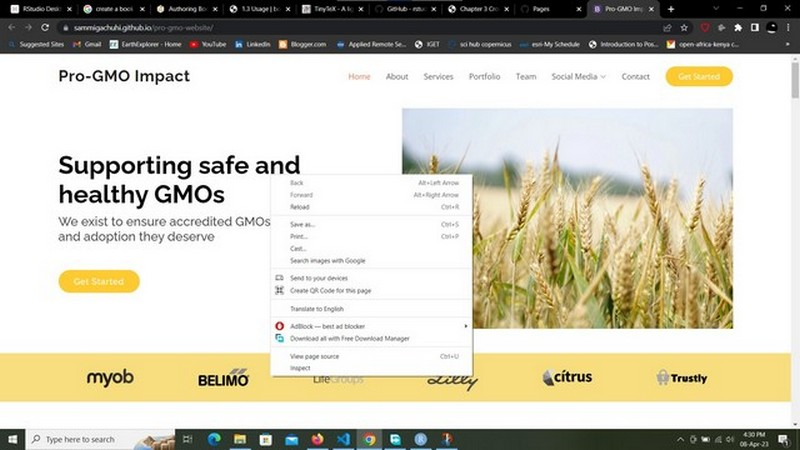
\includegraphics[width=11.11in]{../inspect}

Scroll over to the \textbf{Element} tab and you will have something that looks like this:

\begin{Shaded}
\begin{Highlighting}[]
\NormalTok{knitr}\SpecialCharTok{::}\FunctionTok{include\_graphics}\NormalTok{(}\FunctionTok{rep}\NormalTok{(}\StringTok{"D:/gachuhi/my{-}leaflet/elements.jpg"}\NormalTok{))}
\end{Highlighting}
\end{Shaded}

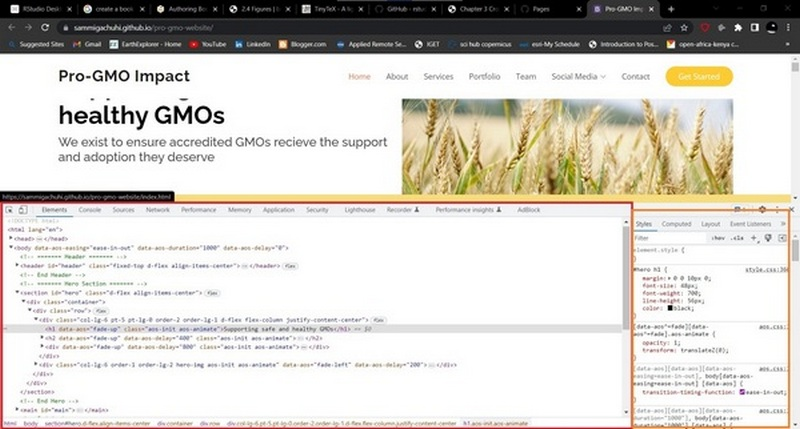
\includegraphics[width=11.11in]{../elements}

The part encircled in red is the \texttt{html} that makes up the webpage for the \href{https://sammigachuhi.github.io/pro-gmo-website/}{ProGMO website} in this case.

So, I am a GIS specialist, I want to learn how to make a html website so as to use leaflet. Whereas this document does not provide an indepth view of a html document, html websites are made up of elements known as \texttt{tags}. Tags, normally indicated by angle brackets (\texttt{\textless{}\textgreater{}}) are what introduce any form of content into a webpage, be it a paragraph \texttt{(\textless{}p\textgreater{})}, an image \texttt{(\textless{}img\textgreater{})}, video \texttt{(\textless{}video\textgreater{})} and even an entire section (\texttt{\textless{}div\textgreater{}}, \texttt{\textless{}section\textgreater{}}, \texttt{\textless{}article\textgreater{}}). With this basic introduction, let's create a basic html page.

To create a html element along with many other programming files, such as \texttt{.js} and \texttt{.css} which we shall see later, we use a text editor. A good example of a text editor is VS code and Pycharm. Check their websites on their installation methods for your personal computer. For this book, we shall be using VS code.

Here is a basic html webpage.

\begin{verbatim}
<!DOCTYPE html>
<html lang="en">
    <head>
        <title>A basic html webpage</title>
        <meta charset="utf-8">
        <link rel="stylesheet" href="style.css">
    </head>
    <body>
        <div id="division-1">
            <p>Hello, World!</p>
        </div>
        <script src="main.js">

        </script>

    </body>
</html>
\end{verbatim}

Let's go through the above tags one by one.

\begin{enumerate}
\def\labelenumi{\arabic{enumi}.}
\item
  \texttt{\textless{}!DOCTYPE\ html\textgreater{}} - It is an ``information'' to the browser about what document type to expect.
\item
  \texttt{\textless{}html\ lang="en"\textgreater{}} - It is the container for all other HTML elements (except for the \textless!DOCTYPE\textgreater{} tag). The \texttt{lang} attribute is used to assist web engines know which language the website uses.
\item
  \texttt{\textless{}head\textgreater{}} - It is not displayed on the webpage as other tags, but contains the metadata of the webpage.
\item
  \texttt{\textless{}title\textgreater{}} - Can you guess? You had it right. Defines the title of the document. In our case, if you open the webpage assuming you created it in VS Code, the webpage shall be titled \emph{A basic html webpage} at the tab of your web-browser.
\item
  \texttt{\textless{}meta\ charset="utf-8"\textgreater{}} - This is one of the metadata hosted by the

  tag. The

  tag defines, rather than contains, as in the case of

  the metadata of the html webpage. In our case, we have used the attribute \texttt{charset="utf-8"} to specify the encoding for HTML5 documents which is \texttt{utf-8}.
\item
  \texttt{\textless{}link\textgreater{}} - Defines the relationship between a document and an external resource. It has various attributes but \texttt{rel} and \texttt{href} have been used. The former specifies the relationship between the current document and the linked document/resource. The \texttt{rel} here references the \texttt{styles.css} file as the style sheet for our html. That is, the styles for our html are found in the \texttt{styles.css} file. \texttt{href} on the other hand points the html document to the path of the stylesheet --the \texttt{styles.css} file.
\item
  \texttt{\textless{}body\textgreater{}} - This is the crux of your webpage. If nothing is within the \texttt{\textless{}body\textgreater{}} tags, your webpage will be as empty as a blank sheet of paper. This tag is the home for all the other contents of the webpage such as headings, paragraphs, images, tables etc.
\item
  \texttt{\textless{}div\textgreater{}} - This is a special element that lets you group similar sets of content together on a web page. You can use it as a generic container for associating similar content. In the above html script, we have included an \texttt{\textless{}id\textgreater{}} attribute that is in other words, a unique identifier for this section of the webpage. \texttt{\textless{}id\textgreater{}s} are useful if you want to customize the appearance of a certain part of the webpage. \texttt{\textless{}class\textgreater{}}es behave in a similar way, but the difference between \texttt{\textless{}id\textgreater{}} and \texttt{\textless{}class\textgreater{}} is that id has to be unique, while \texttt{\textless{}class\textgreater{}}es can be used more than once.
\end{enumerate}

9.\texttt{\textless{}script\textgreater{}} - It is used to embed executable code or data. In most cases it refers to JavaScript, which enhances interactivity.

If you may have noticed above, most HTML tags end with \texttt{\textless{}/name-of-tag\textgreater{}}. With a few exceptions such as \texttt{\textless{}img\textgreater{}}, almost all HTML tags end this way.

\hypertarget{javascript}{%
\section{JavaScript}\label{javascript}}

JavaScript, shortened to \texttt{.js} is the language of the web. It enhances interactivity to HTML files which without it remain just static. Think of \texttt{.js} as the life of the party while HTML is just the setting. Without \texttt{.js} creating webmaps would not be possible since adding them to a html file using \texttt{\textless{}script\textgreater{}} is what brings in the interactive web features to an otherwise blank html.

\hypertarget{css-files}{%
\section{CSS files}\label{css-files}}

CSS stands for \emph{Cascading Style Sheet}. The CSS defines how your HTML is to appear, such as color and size of text, background color of the HTML as well as the structure of your HTML page.

CSS is quite a huge field despite being simple. However, the html elements of a webpage are accompanied by a curly bracket containing the specified properties and values.

\begin{itemize}
\item
  Properties: These are human-readable identifiers that indicate which stylistic features you want to modify. For example, font-size, width, background-color.
\item
  Values: Each property is assigned a value. This value indicates how to style the property.
\end{itemize}

Using the example of our ProGMO website, this is how we would specify the \texttt{\textless{}body\textgreater{}} element of our webpage.

\begin{verbatim}
body {
  font-family: "Open Sans", sans-serif;
  color: #444444;
}
\end{verbatim}

The body is known as the selector. However, selectors can be more specific, such as specifying the exact \texttt{\textless{}div\textgreater{}} that should be displayed in a particular way. Using our html file example, if there were other \texttt{\textless{}div\textgreater{}}s apart from the one above, we would specify our first one in a CSS document like so:

\begin{verbatim}
#division-1 {
  font-family: "Open Sans", sans-serif;
  color: #343a40;
}
\end{verbatim}

The values of that particular \texttt{\textless{}div\textgreater{}} could be changed to whatever you like, so long as they correspond to the right property. If it were a class, the particular class, assuming they were several, would be selected with the convention:

\begin{verbatim}
.class_name {
property: value
prperty2: value2}
\end{verbatim}

You can view the style of a particular HTML element using the styles tab found in the inspect console. It is shown in yellow bounds for a chrome webpage. Firefox should have a similar one.

\begin{Shaded}
\begin{Highlighting}[]
\NormalTok{knitr}\SpecialCharTok{::}\FunctionTok{include\_graphics}\NormalTok{(}\FunctionTok{rep}\NormalTok{(}\StringTok{"D:/gachuhi/my{-}leaflet/elements2.jpg"}\NormalTok{))}
\end{Highlighting}
\end{Shaded}

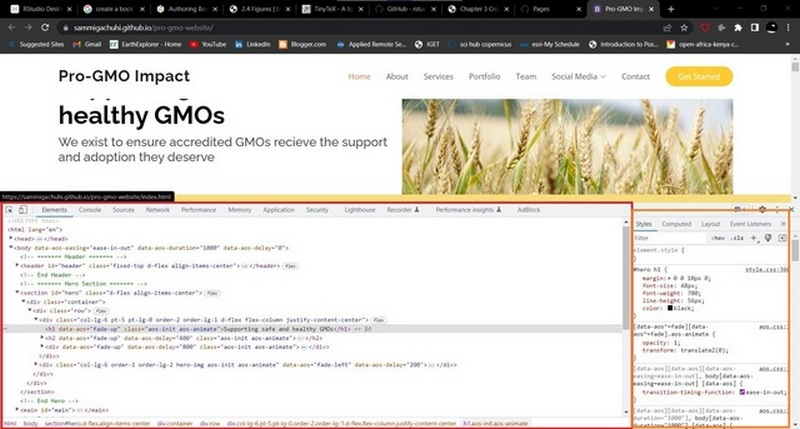
\includegraphics[width=11.11in]{../elements2}

The \href{https://developer.mozilla.org/en-US/docs/Learn/CSS/First_steps/How_CSS_is_structured}{MDN website} provides a lot of information on HTML and CSS.

\begin{Shaded}
\begin{Highlighting}[]
\NormalTok{knitr}\SpecialCharTok{::}\FunctionTok{include\_graphics}\NormalTok{(}\FunctionTok{rep}\NormalTok{(}\StringTok{"https://images.unsplash.com/photo{-}1587404335830{-}7de6dfcff655?ixlib=rb{-}4.0.3\&ixid=MnwxMjA3fDB8MHxwaG90by1wYWdlfHx8fGVufDB8fHx8\&auto=format\&fit=crop\&w=687\&q=80"}\NormalTok{))}
\end{Highlighting}
\end{Shaded}

\includegraphics{https://images.unsplash.com/photo-1587404335830-7de6dfcff655?ixlib=rb-4.0.3\&ixid=MnwxMjA3fDB8MHxwaG90by1wYWdlfHx8fGVufDB8fHx8\&auto=format\&fit=crop\&w=687\&q=80}

\hypertarget{first-leaflet-map}{%
\chapter{First Leaflet Map}\label{first-leaflet-map}}

\hypertarget{setting-the-superstructure}{%
\section{Setting the superstructure}\label{setting-the-superstructure}}

We had earlier mentioned that Javascript, otherwise shorted to JS is the life of the party when it comes to webpages. In other words, it makes your web pages interactive. It's like the additional component that makes you HTML pages move from static to responsive.

Creating a leaflet map is not like creating any other HTML web page. Conventional JS will not do. You have to set up the leaflet essentials in your HTML page first. Create a new html document called \texttt{map.html}. This will be the html document that will act as the structure which will house our webpage to be created using JS. Using VS Code, create \texttt{map.html} and type, or rather, paste the following code.

\begin{verbatim}
<!DOCTYPE html>
<html lang="en">
    <head>
        <title>Leaflet Maps</title>
        <meta charset="utf-8">
        <link rel="stylesheet" href="styles.css">
        <link rel="stylesheet" href="https://unpkg.com/leaflet@1.9.3/dist/leaflet.css"
     integrity="sha256-kLaT2GOSpHechhsozzB+flnD+zUyjE2LlfWPgU04xyI="
     crossorigin=""/>
        <script src="https://unpkg.com/leaflet@1.9.3/dist/leaflet.js"
        integrity="sha256-WBkoXOwTeyKclOHuWtc+i2uENFpDZ9YPdf5Hf+D7ewM="
        crossorigin=""></script>
    </head>
    <body>
        <div id="myMap">
            <script src="main.js">
            </script> 
        </div>  
        
    </body>
</html>
\end{verbatim}

You may be wondering why we have two \texttt{\textless{}link\textgreater{}} tags. ``Won't they confuse the webpage or something?'' You may wonder. Same thing for the two \texttt{\textless{}script\textgreater{}} tags, one at the head and the other at the \texttt{\textless{}body\textgreater{}} tag. The answers is No in terms of confusing and yes in having more than one \texttt{\textless{}link\textgreater{}} tag in a webpage. Once a html script is loaded in our browser, assuming its the \texttt{map.html} we've created, the browser reads it from top to bottom. In our html script, the browser will apply the styles in \texttt{styles.css} to those html elements that have been referenced in that stylesheet. To make matters clearer, the following script is what is contained in the \texttt{styles.css}:

\begin{verbatim}
#myMap { 
    height: 600px; 
}
\end{verbatim}

Therefore, the browser will display everything contained in the \texttt{\textless{}div\textgreater{}} inside the \texttt{\textless{}body\textgreater{}} tag at a height of 500px. This is because the

contains the ID \texttt{myMap} which has been referenced in the local stylesheet as \texttt{\#myMap}. Don't fret about what how things outside the \texttt{\textless{}div\textgreater{}} will be displayed since for our webmap making purposes, hardly will we code anything outside the \texttt{\textless{}div\textgreater{}} tag.

Now to the two \texttt{\textless{}script\textgreater{}} tags. One refers to the online javascript library. The \texttt{src} is in fact linking to a webpage as you can see from the protocol https. The second, housed under the \texttt{\textless{}div\textgreater{}} tag, references to our local javascript file which shall contain all the code to transform our html page to a webmap ninja --lines, polygons and other cool stuff.

\hypertarget{beautifying-the-house}{%
\section{Beautifying the house}\label{beautifying-the-house}}

Think of the html document as the superstructure, like a huge multistorey building just finished. Though the structure has the best architectural design, it just looks all grey with no life unless we call some interior and exterior designers to add some color. That's what \texttt{main.js}, pointed to by the \texttt{\textless{}script\textgreater{}} tag in the html document will precisely do.

Open your VS Code, and assuming you had already created \texttt{main.js} already, (if not, create one now), insert the following code into the \texttt{.js} file.

\begin{verbatim}
var map = L.map('myMap').setView([-0.0884105,34.7299038], 13);;
\end{verbatim}

Take a pause.

Breath in, breath out.

You will learn something very important here. In fact, it is the crux of what makes Leaflet work. Your future of understanding leaflet hinges on this code.

The \texttt{L.map()} class we just used is what initializes the leaflet map. Everything within the \texttt{\textless{}div\textgreater{}} is displayed thanks to this class function. It is referred to as a factory function because it uses the method \texttt{map} to return an object.

The \texttt{setView} method \emph{sets the view of the map (geographical center and zoom) with the given animation options}. It's properties are Latitude-Longitude, zoom number and other options. If you would like to view the humungous leaflet reference, get it \href{https://leafletjs.com/reference.html}{here}.

In our case we just inserted the Lat-Long and zoom number.

Try loading your \texttt{map.html}. All you see is a grey canvas with zoom options. This is because we haven't added a tilelayer yet. A \href{https://pro.arcgis.com/en/pro-app/latest/help/data/services/use-tiled-web-layers.htm}{tileLayer} is a set of web-accessible tiles that reside on a server. A tile is an individual image or vector file from a server which are collectively joined together to form the webmap. If you've zoomed into a webmap, say Google Maps and noticed boxes appearing as you zoomed in or out, those are \emph{tiles}.

Let's load an example of a common tile layer, the Open StreetMap into Leaflet.

\begin{verbatim}
L.tileLayer('https://tile.openstreetmap.org/{z}/{x}/{y}.png', {
    maxZoom: 19,
    attribution: '&copy; <a href="http://www.openstreetmap.org/copyright">OpenStreetMap</a>'
}).addTo(map);
\end{verbatim}

Reload your html page again. What do you see?

\begin{Shaded}
\begin{Highlighting}[]
\NormalTok{knitr}\SpecialCharTok{::}\FunctionTok{include\_graphics}\NormalTok{(}\FunctionTok{rep}\NormalTok{(}\StringTok{"D:/gachuhi/my{-}leaflet/kisumu{-}leaflet.jpg"}\NormalTok{))}
\end{Highlighting}
\end{Shaded}

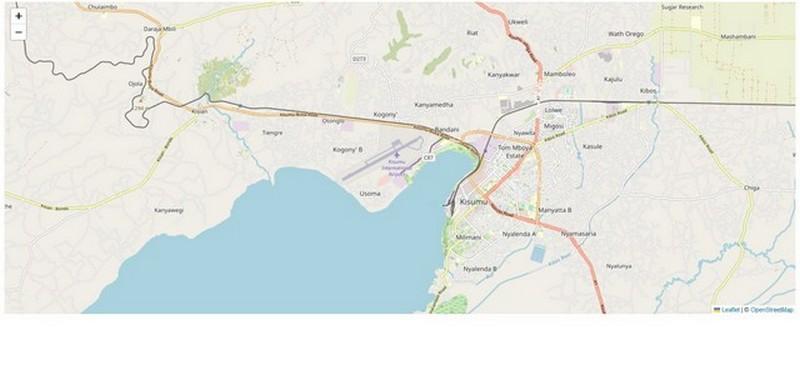
\includegraphics[width=11.11in]{../kisumu-leaflet}

What \texttt{L.tileLayer} has done is retrieve the web tiles from the url source provided, and within the dictionary, zoom and attribution have been provided. When working with leaflet, the dictionary, indicated by the curly braces \texttt{\{\}} houses most of the additional class options other than the key one(s). In this case we used the additional options of \texttt{maxZoom} and \texttt{attribution}. Finally, the method \texttt{addTo} adds the layer to the given map or layer group. Here, or webtile is added to the \texttt{var\ map} which only contains the \texttt{setView} properties.

A very influential person said Kisumu located in Kenya is a town with great potential. How about dispalying it to the whole world to realist it!

\begin{Shaded}
\begin{Highlighting}[]
\NormalTok{knitr}\SpecialCharTok{::}\FunctionTok{include\_graphics}\NormalTok{(}\FunctionTok{rep}\NormalTok{(}\StringTok{"https://images.unsplash.com/photo{-}1515898913320{-}f38370edab7a?ixlib=rb{-}4.0.3\&ixid=MnwxMjA3fDB8MHxwaG90by1yZWxhdGVkfDEwfHx8ZW58MHx8fHw\%3D\&auto=format\&fit=crop\&w=600\&q=60"}\NormalTok{))}
\end{Highlighting}
\end{Shaded}

\includegraphics{https://images.unsplash.com/photo-1515898913320-f38370edab7a?ixlib=rb-4.0.3\&ixid=MnwxMjA3fDB8MHxwaG90by1yZWxhdGVkfDEwfHx8ZW58MHx8fHw\%3D\&auto=format\&fit=crop\&w=600\&q=60}

\hypertarget{add-ons}{%
\chapter{Add ons}\label{add-ons}}

So we have a plain looking webmap like the one shown below.

\begin{Shaded}
\begin{Highlighting}[]
\NormalTok{knitr}\SpecialCharTok{::}\FunctionTok{include\_graphics}\NormalTok{(}\FunctionTok{rep}\NormalTok{(}\StringTok{"D:/gachuhi/my{-}leaflet/kisumu{-}leaflet.jpg"}\NormalTok{))}
\end{Highlighting}
\end{Shaded}

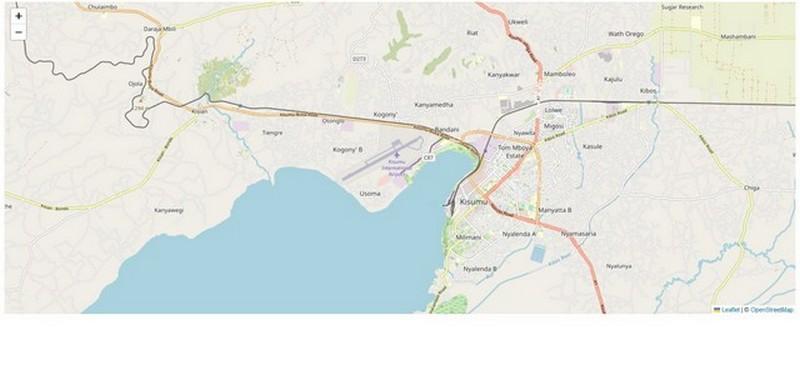
\includegraphics[width=11.11in]{../kisumu-leaflet}

However, though a cool looking webmap, it offers no sort of information to the viewer except that it is an interactive map interface. In order to create some information, such as the location of Kisumu and other features you want to highlight, markers are one way of displaying this kind of information.

First things, first, we had last left our \texttt{main.js} file looking like this. Ensure yours is also the same, but we encourage to explore with other leaflet layers available from \href{https://leaflet-extras.github.io/leaflet-providers/preview/}{here}.

\hypertarget{a-marker}{%
\section{A marker}\label{a-marker}}

Many people could possible not know where Kisumu, is, so lets indicate its location with a simple pin marker. To be more specific since the name Kisumu may infer a large area, let's pinpoint Kisumu International Airport.

\begin{verbatim}
// Location of Kisumu International Airport
var marker = L.marker([-0.0819301, 34.7260167]).addTo(map);
\end{verbatim}

\begin{Shaded}
\begin{Highlighting}[]
\NormalTok{knitr}\SpecialCharTok{::}\FunctionTok{include\_graphics}\NormalTok{(}\FunctionTok{rep}\NormalTok{(}\StringTok{"D:/gachuhi/my{-}leaflet/kisumu{-}international{-}airport.jpg"}\NormalTok{))}
\end{Highlighting}
\end{Shaded}

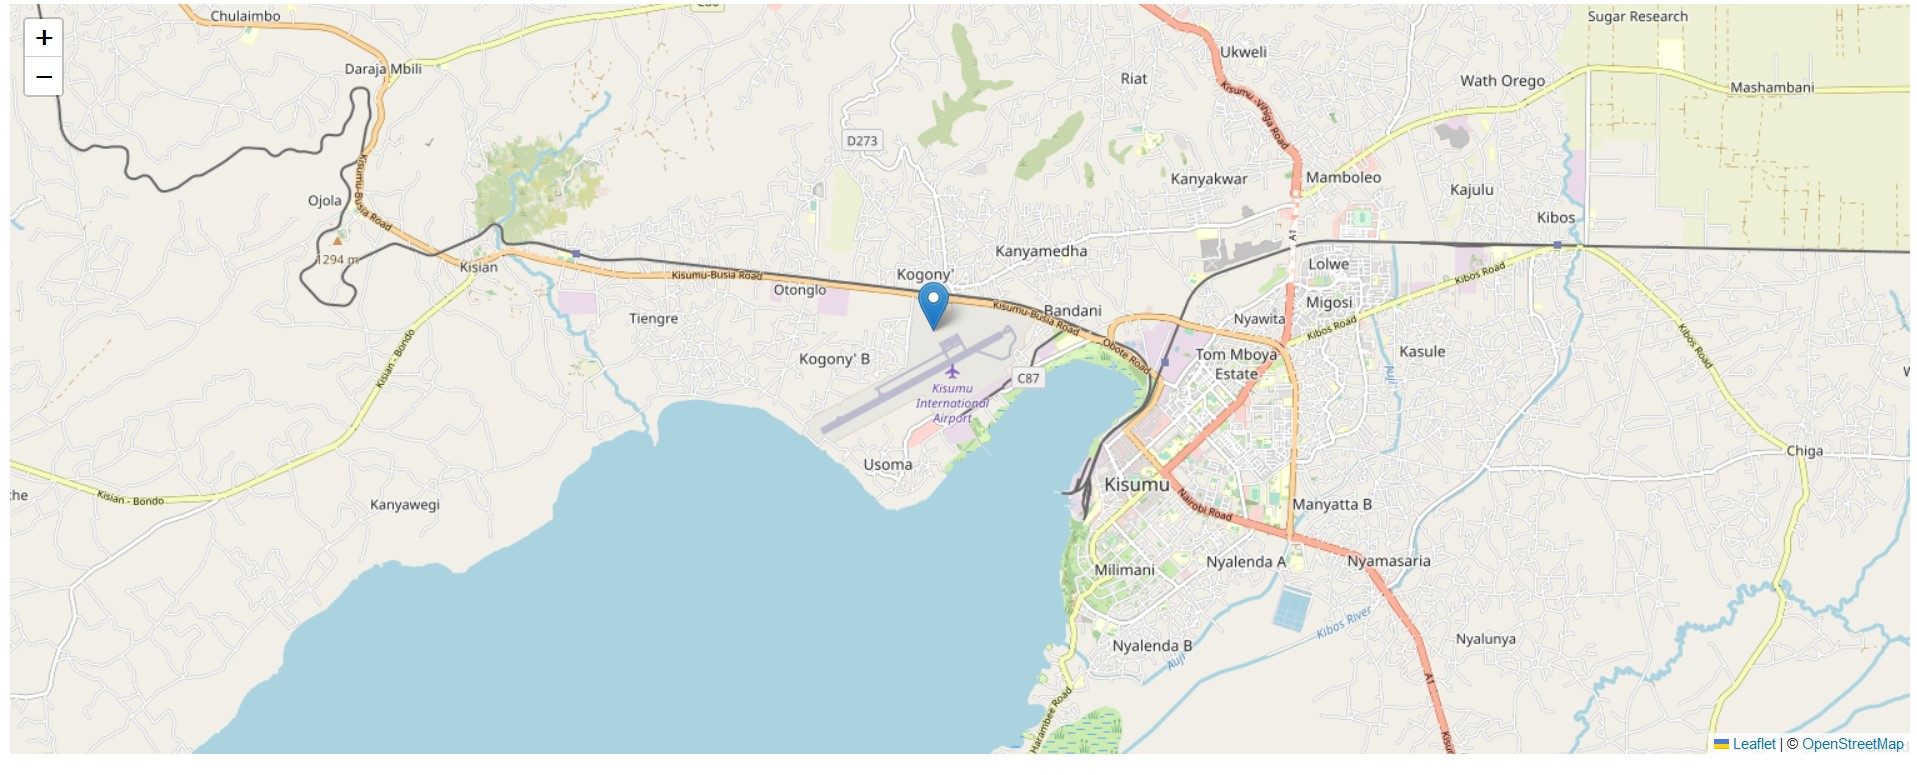
\includegraphics[width=26.62in]{../kisumu-international-airport}

Can you try creating a marker for your home location, not forgetting to change the \texttt{setView} method you had initially started with in this map creating journey?

Alright, we have a marker. But as they say, going the extra mile is what counts in both the corporate as well as personal goals. Let's try to make this marker have some information, called attributes in GIS, of um, let's say the name of the airport and other auxillary data.

\hypertarget{a-marker-with-a-popup}{%
\section{A marker with a popup}\label{a-marker-with-a-popup}}

To create popups, leaflet provides the \texttt{bindPopup} method. It is especially easy if you already have a marker variable in place, as in our case. Let's exploit this advantage.

\begin{verbatim}
// Create popup of Kisumu international Airport
marker.bindPopup("Kisumu International Airport.").openPopup();
\end{verbatim}

\begin{Shaded}
\begin{Highlighting}[]
\NormalTok{knitr}\SpecialCharTok{::}\FunctionTok{include\_graphics}\NormalTok{(}\FunctionTok{rep}\NormalTok{(}\StringTok{"D:/gachuhi/my{-}leaflet/kisumu{-}airport{-}popup.jpg"}\NormalTok{))}
\end{Highlighting}
\end{Shaded}

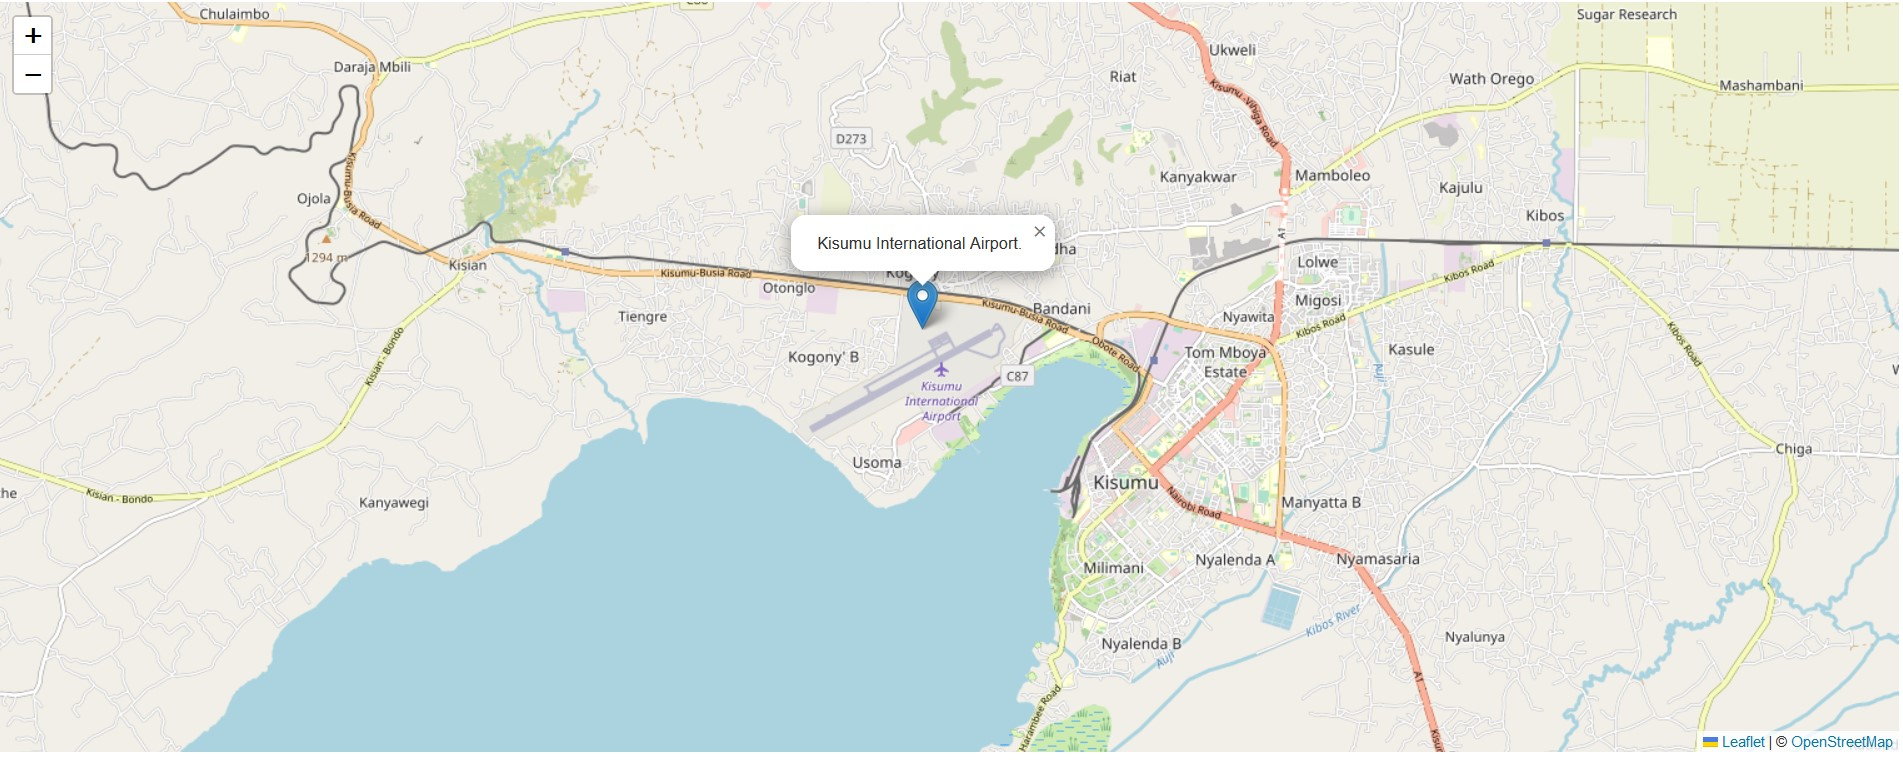
\includegraphics[width=26.43in]{../kisumu-airport-popup}

What has just happened is that \texttt{bindPopup} binds the popup content ``Kisumu International Airport'' to the marker. The following \texttt{popUp} method chained to the method \emph{opens} the popup at that specified latitude longitude. If you remove, or comment \texttt{//} out the \texttt{popuUp} method, you will have to click the marker to see the popup content. Try it out.

Markers can also work with hmtl elements, such as when you want to display additional metadata, say the owner of the place, size of land et ceterra. In the below case, we have added the lat-lon coordinates of Kisumu airport location. I would advise not to include lengthy information in an HTML marker element.

\begin{verbatim}
// With html content
marker.bindPopup("<br>Name: Kisumu International Airport</br><br>Latitude: -0.0819301</br><br>Longitude: 34.7260167</br>").openPopup();
\end{verbatim}

\begin{Shaded}
\begin{Highlighting}[]
\NormalTok{knitr}\SpecialCharTok{::}\FunctionTok{include\_graphics}\NormalTok{(}\FunctionTok{rep}\NormalTok{(}\StringTok{"D:/gachuhi/my{-}leaflet/marker{-}html.jpg"}\NormalTok{))}
\end{Highlighting}
\end{Shaded}

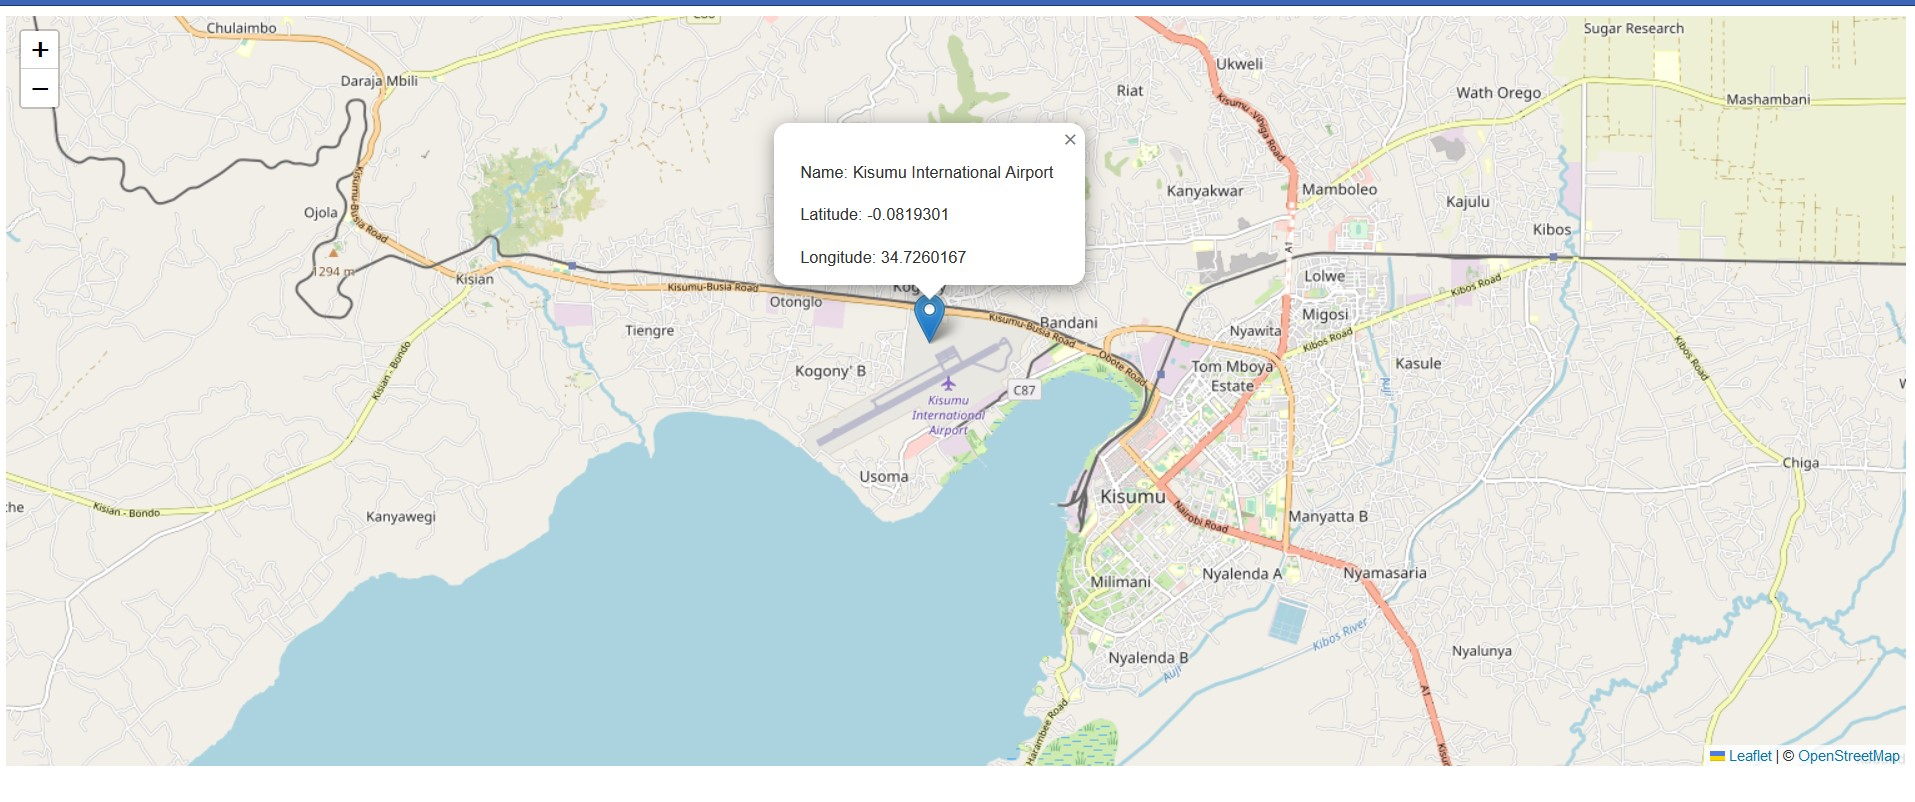
\includegraphics[width=26.6in]{../marker-html}

\hypertarget{other-markers-and-different-popup-creation-methods}{%
\section{Other markers and different popup creation methods}\label{other-markers-and-different-popup-creation-methods}}

So far you have seen pin markers, but there are also other kinds of markers, circles and rectangles even. Unlike the pin markers we have been experimenting with, these other markers require additional options, such as radius for circle and lat-long cooordinates for rectangles. Let's have a go with each.

Starting with a circle, let's start by inserting a circle to show the location of Kisumu Museum.

\begin{verbatim}
// Circle over Kisumu Museum
var circle = L.circle([-0.107637, 34.7435975]).setRadius(2000).addTo(map);
\end{verbatim}

\begin{Shaded}
\begin{Highlighting}[]
\NormalTok{knitr}\SpecialCharTok{::}\FunctionTok{include\_graphics}\NormalTok{(}\FunctionTok{rep}\NormalTok{(}\StringTok{"D:/gachuhi/my{-}leaflet/kisumu{-}museum{-}circle.jpg"}\NormalTok{))}
\end{Highlighting}
\end{Shaded}

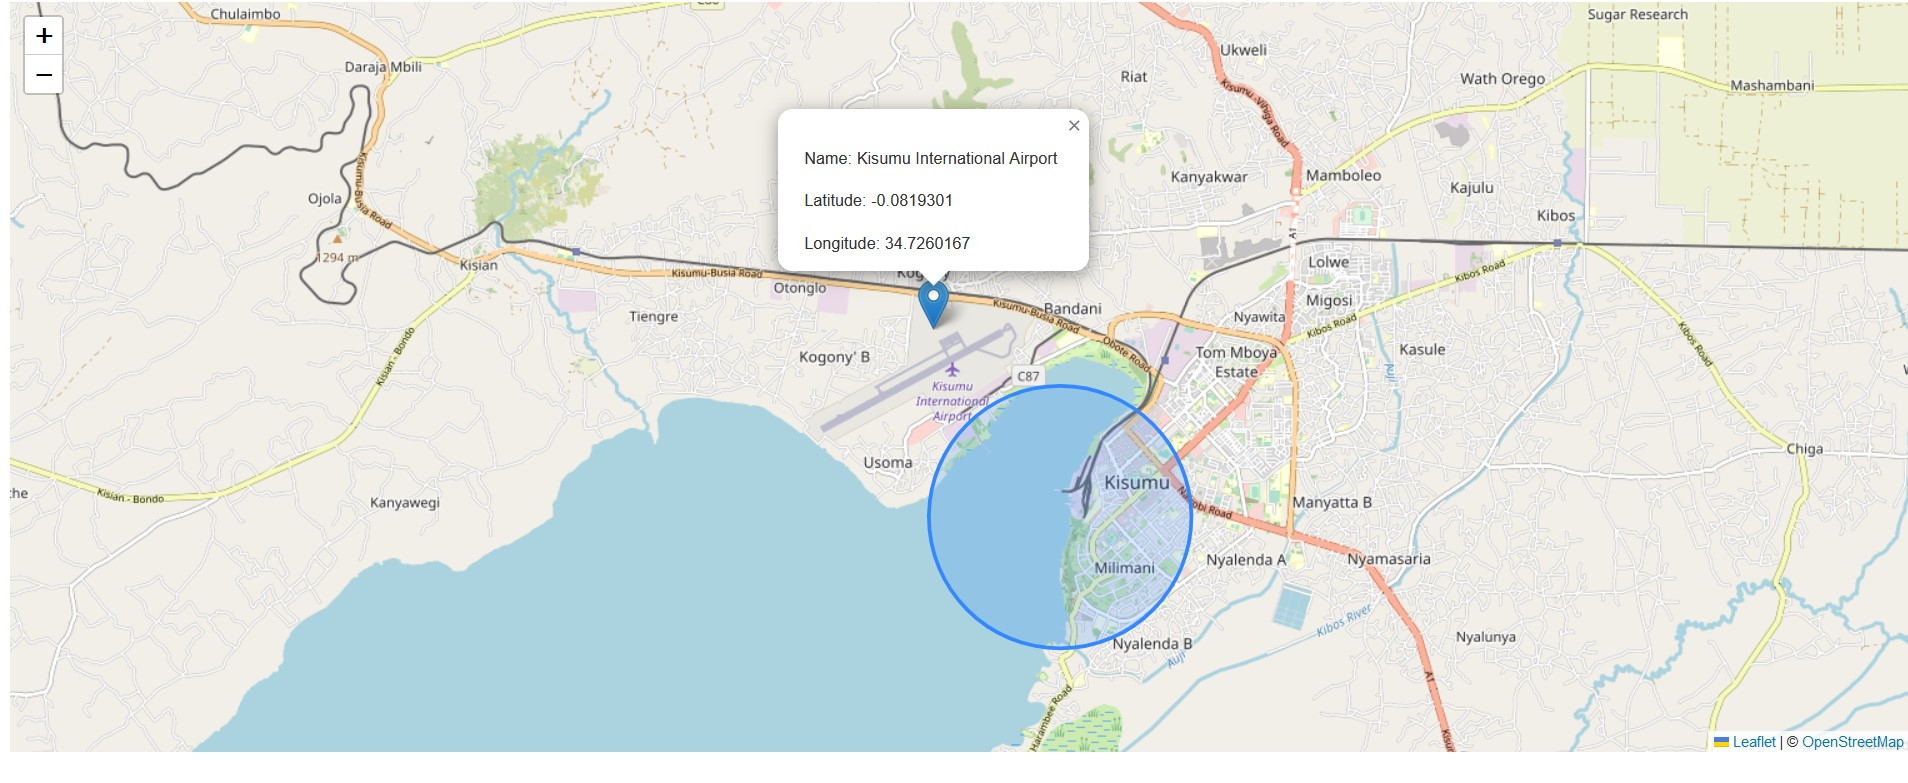
\includegraphics[width=26.5in]{../kisumu-museum-circle}

The below code will also create a slightly similar circle marker, the only difference is that in the preceding one we didn't insert \texttt{\{options\}} and we set radius using the \texttt{setRadius} method. In the second one below, we have been very specific in what we want --our specifications going into the curly brackets \{\} before adding the circle marker to our map. Brackets in javascript denote \href{https://flexiple.com/javascript/javascript-dictionary/}{dictionaries}. Dictionaries in javascript and even in python are used to denote key-value pairs. Best for look-ups.

\begin{verbatim}
var circle = L.circle([-0.107637, 34.7435975], {
    color: 'blue',
    fillColor: 'blue',
    fillOpacity: .5,
    radius: 2000
}).addTo(map);
\end{verbatim}

As we had mentioned earlier, other marker elements such as circles and rectangles can have popups attached to them. Ready for something cool, we will attach a popup into our circle. Not just any other ordinary hard coded popup but one in which relies on other methods to generate an output. In our case, we want a pop up that shows the radius of our circle without necessarily typing it in.

\begin{verbatim}
// Circle marker pop up for Kisumu Museum
var getRadius = circle.getRadius();
circle.bindPopup("Radius is: " + getRadius.toString() + " metres");
\end{verbatim}

In our above code, \texttt{getRadius} gets the radius of our circle marker. \texttt{bindPopup} has it has already been severally explained \emph{binds} the popup content to our circle marker. But there is a catch. The variable \texttt{getRadius} is used to print out the results, which is 2000 of course. However, \texttt{bindPopup} only understands strings so we convert our variable result to a string using \texttt{toString()}. We also added other strings to give the popup a wholesome result that is understandable to every Tom, Dick, Harry and Harriet.

\begin{Shaded}
\begin{Highlighting}[]
\NormalTok{knitr}\SpecialCharTok{::}\FunctionTok{include\_graphics}\NormalTok{(}\FunctionTok{rep}\NormalTok{(}\StringTok{"D:/gachuhi/my{-}leaflet/circle{-}radius.jpg"}\NormalTok{))}
\end{Highlighting}
\end{Shaded}

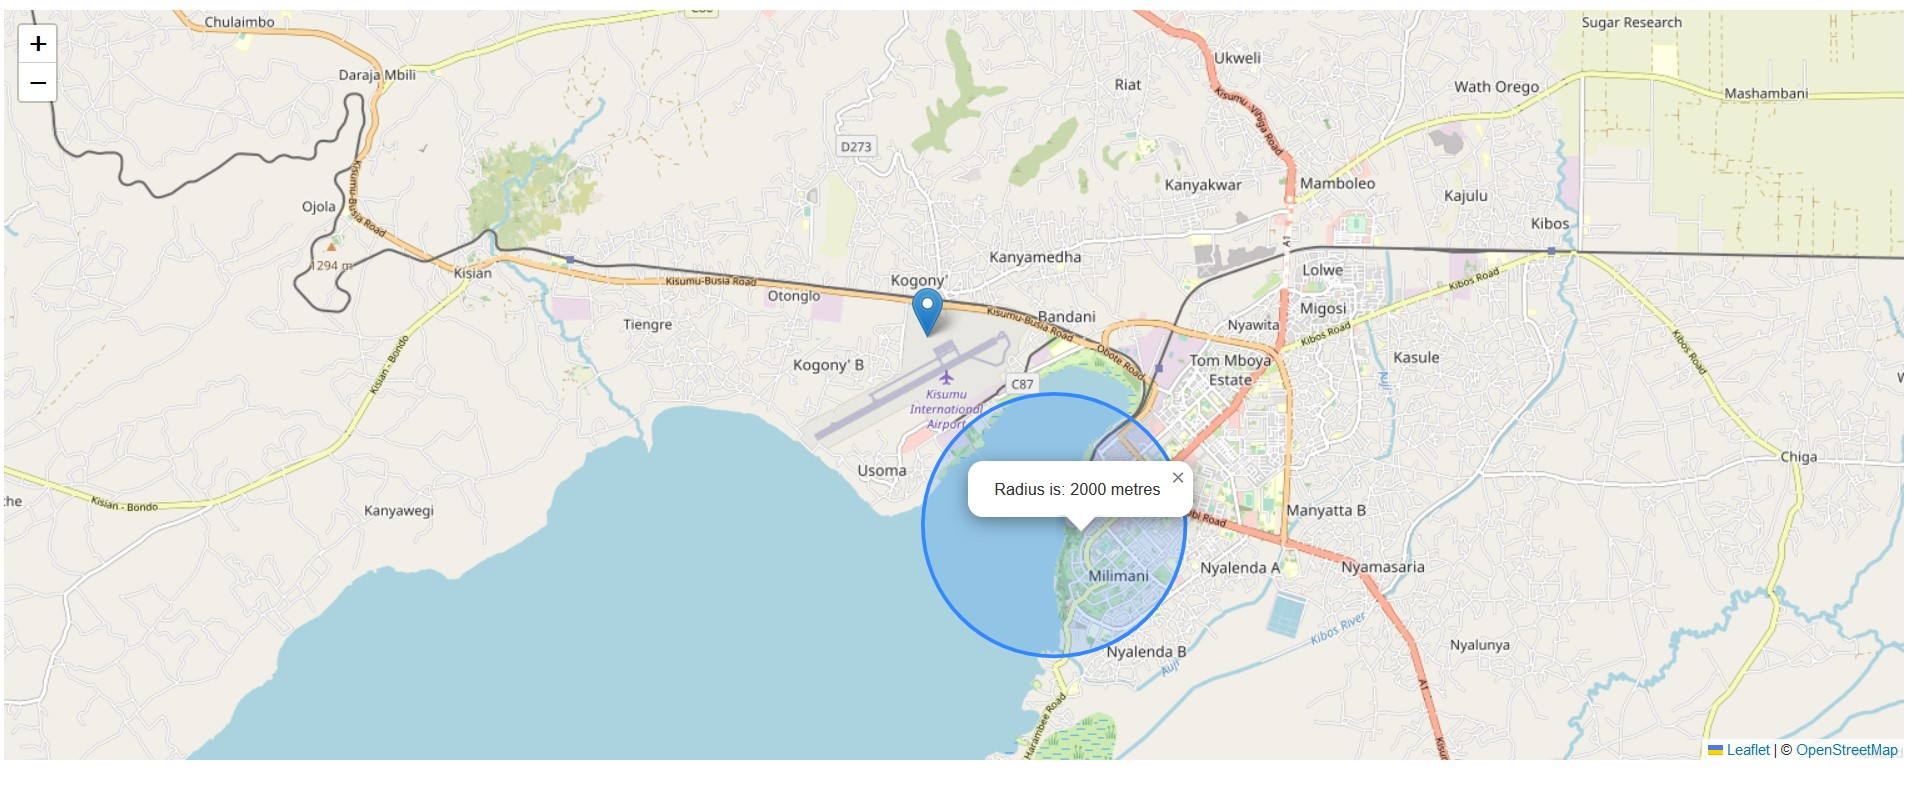
\includegraphics[width=26.57in]{../circle-radius}

Finally, let's try with a rectangle. Actually, leaflet allows us to create polygons, and with a polygon, you can also create rectangles. Let's work with the polygon class instead.

Copy the following coordinates.

\begin{verbatim}
// Draw rectangle around Kisumu Wildlife Impala Park
var impalaParkCoordinates = [
    [-0.1144753, 34.743418],
    [-0.115097, 34.745242],
    [-0.114238, 34.745071],
    [-0.114002, 34.746101],
    [-0.115054, 34.746787],
    [-0.115998, 34.745586],
    [-0.118444, 34.746208],
    [-0.121255, 34.744684]
]
\end{verbatim}

Now using the \texttt{L.polygon} class and a few optional parameters, let's showcase where the Kisumu Wildlife Impala Park is situated.

\begin{verbatim}
// Create a polygon using the above coordinates
var impalaParkPolygon = L.polygon(impalaParkCoordinates, {
    color: 'brown',
    fillOpacity: 0.4
}).addTo(map);
\end{verbatim}

You will notice that the Kisumu Museum circle overlaps the location of the Kisumu Impala Park but that is no problem. We will make our popup content appear by default as soon as you load the map. Just like we did for the circle marker, we will make our popup content rely on another variable, in this case \texttt{getCenter} which gets the centroid coordinates of our polygon. We were looking for something cooler such as \texttt{getArea} but we were unable to find it.

\begin{verbatim}
// Add popup to the polygon of Kisumu Impala Park
var getCenter = impalaParkPolygon.getCenter();
impalaParkPolygon.bindPopup("Centre is at Lat-Lon: " + getCenter.toString()).openPopup();
\end{verbatim}

If you find the circle marker radius too obstracting you can comment out it and its dependancies using \texttt{//}.

\begin{Shaded}
\begin{Highlighting}[]
\NormalTok{knitr}\SpecialCharTok{::}\FunctionTok{include\_graphics}\NormalTok{(}\FunctionTok{rep}\NormalTok{(}\StringTok{"D:/gachuhi/my{-}leaflet/polygon{-}marker.jpg"}\NormalTok{))}
\end{Highlighting}
\end{Shaded}

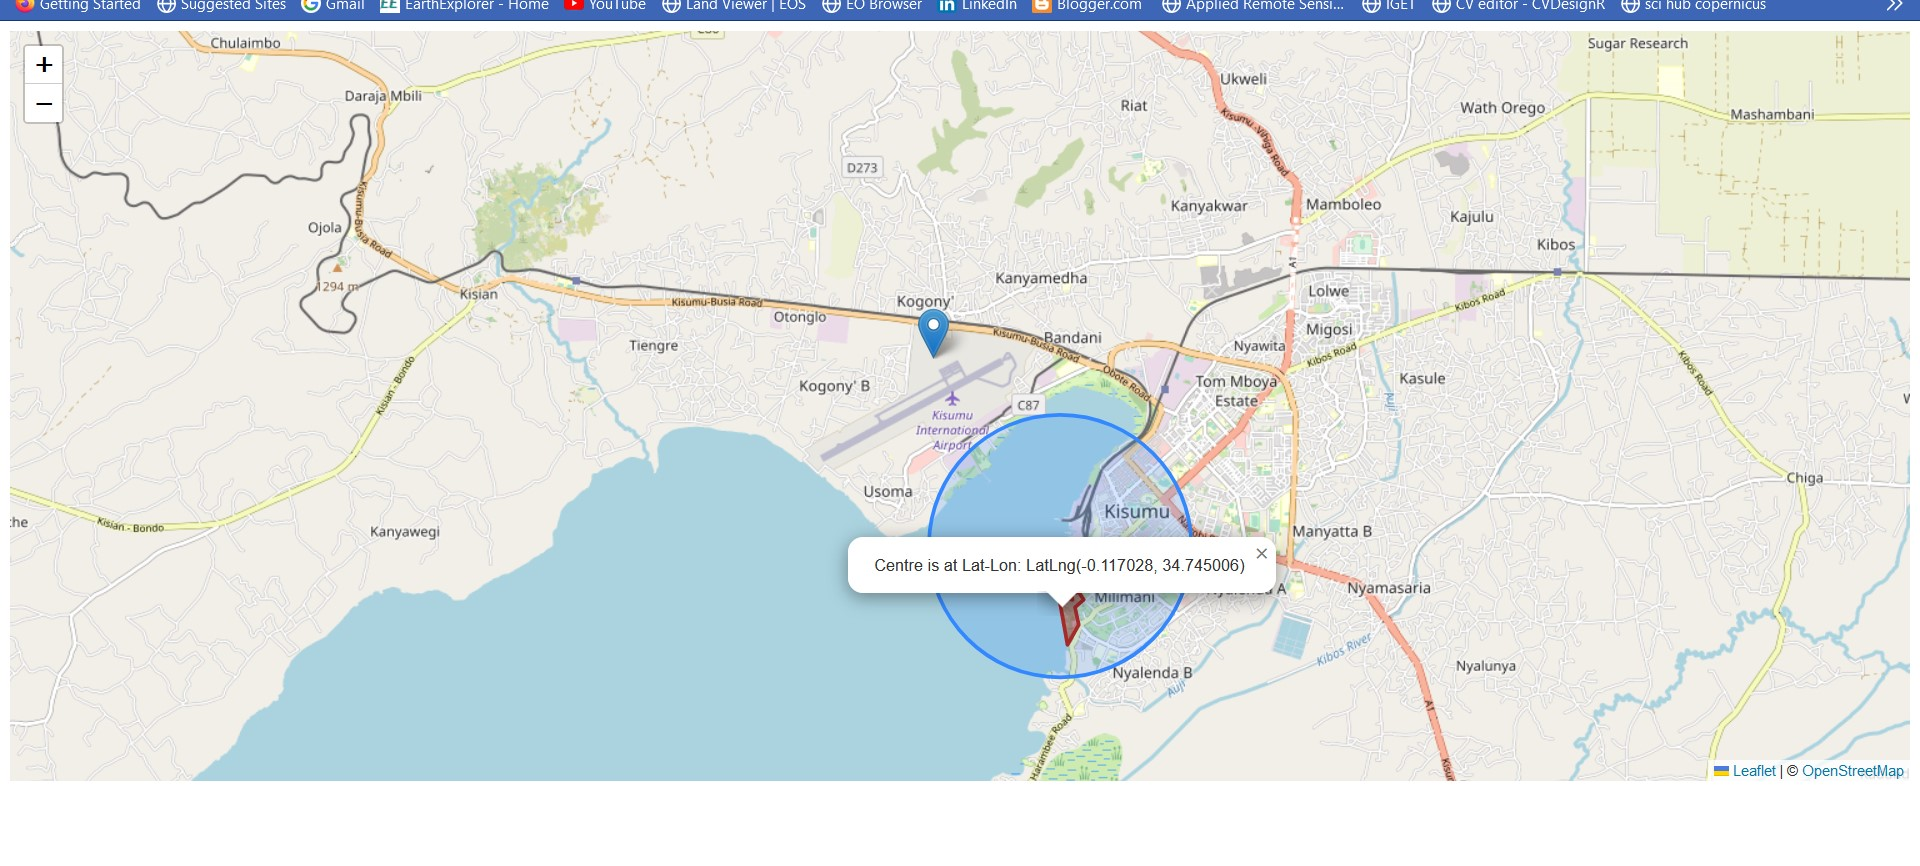
\includegraphics[width=26.67in]{../polygon-marker}

You can get the files used in this exercise \href{https://www.dropbox.com/scl/fo/qznia963vaq8s4ca51p51/h?dl=0\&rlkey=glj4ew599c4v9fikq11wn1fje}{here}.

\begin{Shaded}
\begin{Highlighting}[]
\NormalTok{knitr}\SpecialCharTok{::}\FunctionTok{include\_graphics}\NormalTok{(}\FunctionTok{rep}\NormalTok{(}\StringTok{"https://images.unsplash.com/photo{-}1609848930155{-}cd505cf3cd38?ixlib=rb{-}4.0.3\&ixid=MnwxMjA3fDB8MHxwaG90by1wYWdlfHx8fGVufDB8fHx8\&auto=format\&fit=crop\&w=1170\&q=80"}\NormalTok{))}
\end{Highlighting}
\end{Shaded}

\includegraphics{https://images.unsplash.com/photo-1609848930155-cd505cf3cd38?ixlib=rb-4.0.3\&ixid=MnwxMjA3fDB8MHxwaG90by1wYWdlfHx8fGVufDB8fHx8\&auto=format\&fit=crop\&w=1170\&q=80}

\hypertarget{embedding-leaflet-map-to-an-external-website}{%
\chapter{Embedding leaflet map to an external website}\label{embedding-leaflet-map-to-an-external-website}}

Now, we have succeeded in making a stand alone leaflet map. However, we want to do something that will upscale from a novice to a pro. That is, we just do one leaflet exercise that will give us that entry to the IT department. If we convince our boss that we could embed a webmap of their branch locations, they could consider us a webmapping guru rather than just another cog in the organization's wheel.

An example of what we want is shown below, which is a snapshot from the \href{https://data.humdata.org/dataset/cod-ab-ken}{HDX website}.

\begin{Shaded}
\begin{Highlighting}[]
\NormalTok{knitr}\SpecialCharTok{::}\FunctionTok{include\_graphics}\NormalTok{(}\FunctionTok{rep}\NormalTok{(}\StringTok{"D:/gachuhi/my{-}leaflet/webmap{-}in{-}web.jpg"}\NormalTok{))}
\end{Highlighting}
\end{Shaded}

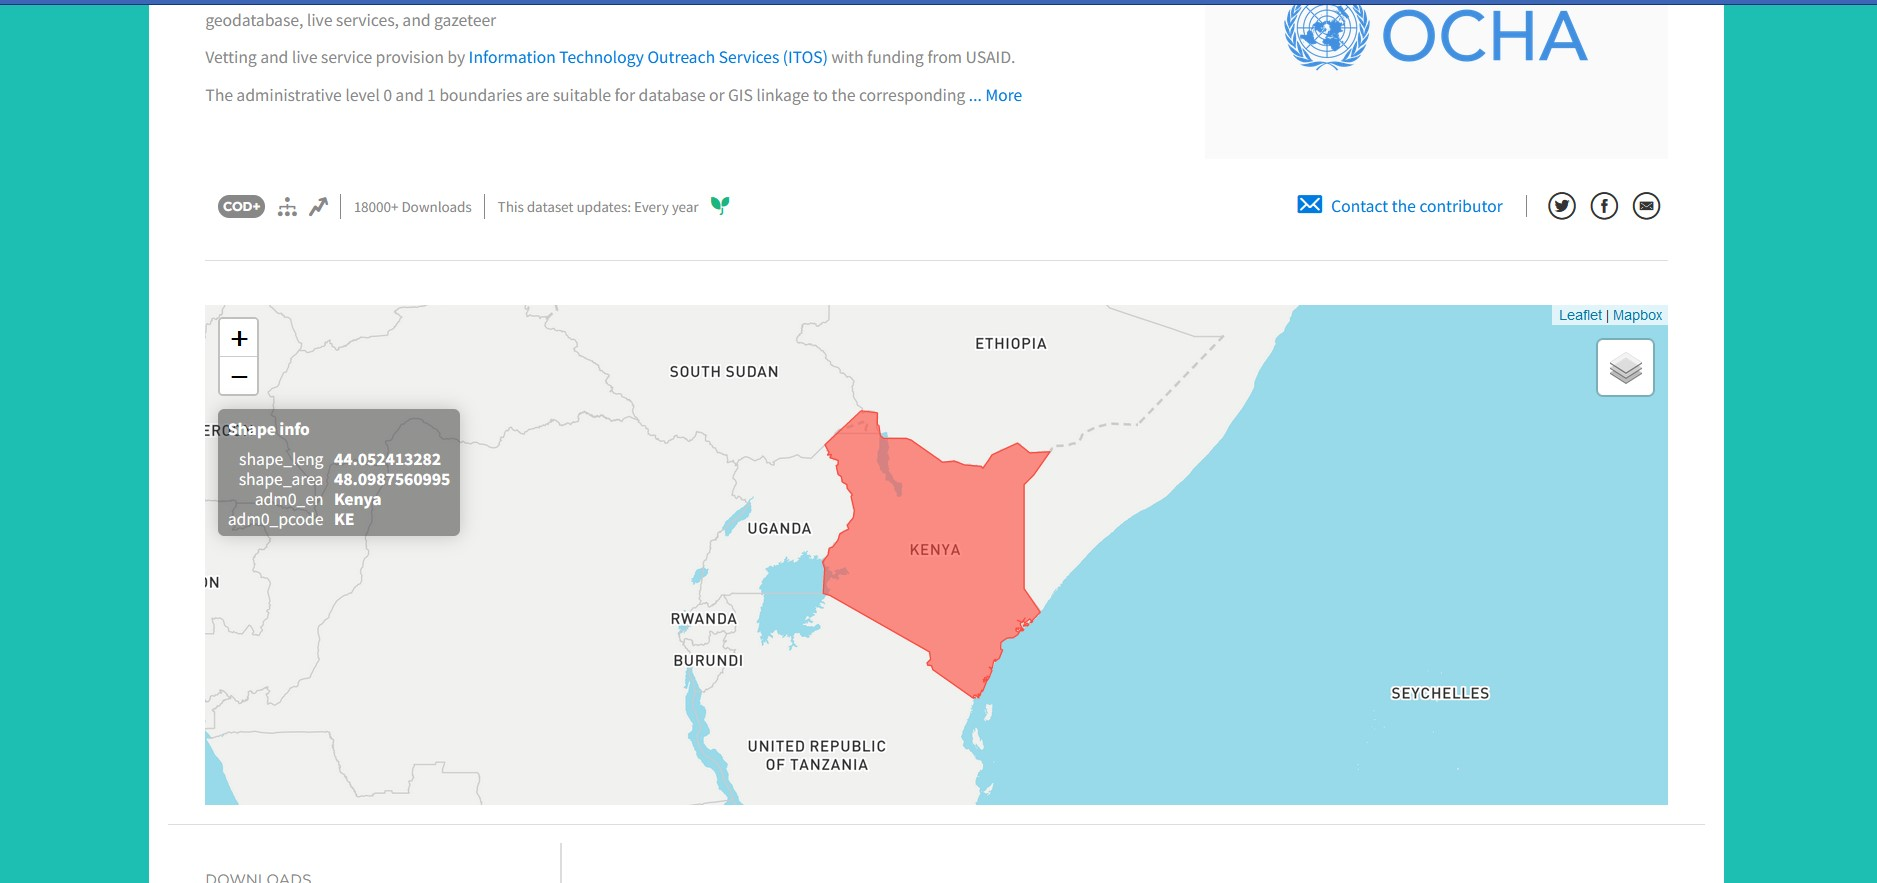
\includegraphics[width=26.07in]{../webmap-in-web}

For this exercise, we shall embed a leaflet map to a simple html webpage. This webpage doesn't look grand, but it serves the purpose of our exercise. Let's get on to it. Here are the \href{https://www.dropbox.com/scl/fo/2u5xzr83z08rfxnlh8pc9/h?dl=0\&rlkey=zcrui1dsi7fzi3s5891yx9rty}{files}.

\hypertarget{the-html-webpage}{%
\section{The html webpage}\label{the-html-webpage}}

Create a html page with the following code.

\begin{verbatim}
<!DOCTYPE html>
<html lang="en">
    <head>
        <title>Pro-GMO Alliance</title>
        <meta charset="utf-8">
        <link rel="stylesheet" href="example-styles.css">
        <link rel="stylesheet" href="https://unpkg.com/leaflet@1.9.3/dist/leaflet.css"
        integrity="sha256-kLaT2GOSpHechhsozzB+flnD+zUyjE2LlfWPgU04xyI="
        crossorigin=""/>
        <script src="https://unpkg.com/leaflet@1.9.3/dist/leaflet.js"
        integrity="sha256-WBkoXOwTeyKclOHuWtc+i2uENFpDZ9YPdf5Hf+D7ewM="
        crossorigin=""></script>
    </head>
    <body>
    <div id="div-for-article">
        <article id="introduction">
            <h2>Introduction</h2>
            <q>Sed ut perspiciatis unde omnis iste natus error sit voluptatem accusantium 
            doloremque laudantium, totam rem aperiam, eaque ipsa quae ab illo inventore veritatis et 
            quasi architecto beatae vitae dicta sunt explicabo. Nemo enim ipsam voluptatem quia voluptas 
            sit aspernatur aut odit aut fugit, sed quia consequuntur magni dolores eos qui ratione 
            voluptatem sequi nesciunt. Neque porro quisquam est, qui dolorem ipsum quia dolor sit amet, 
            consectetur, adipisci velit, sed quia non numquam eius modi tempora incidunt ut labore et 
            dolore magnam aliquam quaerat voluptatem. Ut enim ad minima veniam, quis nostrum exercitationem 
            ullam corporis suscipit laboriosam, nisi ut aliquid ex ea commodi consequatur? Quis autem 
            vel eum iure reprehenderit qui in ea voluptate velit esse quam nihil molestiae consequatur, 
            vel illum qui dolorem eum fugiat quo voluptas nulla pariatur?</q>
        </article>
    </div>
    <div id="div-for-section">
        <section id="Products">
            <div class="row">
                <h2>Our Products</h2>
                <div class="column">
                  <img src="https://images.unsplash.com/photo-1632125941710-35a9d2fcc7ce?ixlib=rb-4.0.3&ixid=MnwxMjA3fDB8MHxwaG90by1wYWdlfHx8fGVufDB8fHx8&auto=format&fit=crop&w=1170&q=80" alt="Maize" style="width:100%">
                </div>
                <div class="column">
                    <img src="https://images.unsplash.com/photo-1595615636850-3292eb0a95b0?ixlib=rb-4.0.3&ixid=MnwxMjA3fDB8MHxwaG90by1wYWdlfHx8fGVufDB8fHx8&auto=format&fit=crop&w=1170&q=80" alt="Sunflower" style="width:100%">
                  </div>
                <div class="column">
                  <img src="https://images.unsplash.com/photo-1600333859399-228aa03f7dba?ixlib=rb-4.0.3&ixid=MnwxMjA3fDB8MHxwaG90by1wYWdlfHx8fGVufDB8fHx8&auto=format&fit=crop&w=1170&q=80" alt="Potato" style="width:100%">
                </div>
                <div class="column">
                  <img src="https://images.unsplash.com/photo-1630145398476-853543b02843?ixlib=rb-4.0.3&ixid=MnwxMjA3fDB8MHxwaG90by1wYWdlfHx8fGVufDB8fHx8&auto=format&fit=crop&w=1167&q=80" alt="Cotton" style="width:100%">
                </div>
              </div>
        </section>
    </div>
    <div>
        <br>
        <h2>Our Branches</h2>
        <br>
    </div>
      <div class="container">
        <div id="map">
          <script src="example-main.js"></script>
        </div>
        <div class="text">
          <h1>Address</h1>
          <p>
            P.O. Box 55044, Nakuru
        </p>
        </div>
      </div>
    </body>
</html>
\end{verbatim}

Since this is a geospatial book, we shall not go through every line of the HTML code above. It just a webpage containing some text, some pictures and a webmap. The webmap is the centre of our interest. How do we create a Leaflet map, of which we know how to do it, and fit it inside an existing webpage?

\hypertarget{the-css}{%
\section{The CSS}\label{the-css}}

Before we head there, let's insert the CSS file, which looks like this.

\begin{verbatim}
/* Three image containers (use 25% for four, and 50% for two, etc) */
.column {
    float: left;
    width: 33.33%;
    padding: 5px;
  }
  
  /* Clear floats after image containers */
  .row::after {
    content: "";
    clear: both;
    display: table;
  }


/* Styling the map */
  .container {
    display: flex;
    align-items: center;
    justify-content: center
  }

#map {
    height: 300px; 
    width: 90%
}

.text {
    font-size: 15px;
    padding-left: 20px;
}
\end{verbatim}

\hypertarget{the-leaflet-js-code-for-our-website}{%
\section{The leaflet js code for our website}\label{the-leaflet-js-code-for-our-website}}

Back to the leaflet map of our dummy Pro-GMO Alliance webpage. How did we put the leaflet in there. Nothing complicated, just inserting the same leaflet code, with some additional javascript and referencing it within the html file with \texttt{\textless{}script\ src="example-main.js"\textgreater{}\textless{}/script\textgreater{}}. The Javascript file used is shown below.

\begin{verbatim}
var map = L.map('map').setView([-0.302765, 36.146147], 12);

L.tileLayer('https://tile.openstreetmap.org/{z}/{x}/{y}.png', {
    maxZoom: 19,
    attribution: '&copy; <a href="http://www.openstreetmap.org/copyright">OpenStreetMap</a>'
}).addTo(map);

var branches = [
    ["Potatoes",-0.328858, 36.008474],
    ["Maize",-0.302765, 36.146147],
    ["Sunflower",-0.224832, 36.159880],
    ["Cotton", -0.214189, 36.135847]
    ];

for (var i = 0; i < branches.length; i++) {
    marker = new L.marker([branches[i][1], branches[i][2]])
        .bindPopup(branches[i][0])
        .addTo(map);
}
\end{verbatim}

The only new thing in the above script is the \texttt{for} loop. In javascript, the \texttt{for} loop is used to iterate over items. In this case, and remembering that indexing in javascript arrays begins from 0 just is does for Python, the marker popups will read the latitudes and longitudes which are at index 1 and 2 respectively. The popup strings, which appear as the first elements in the \texttt{branches} array, are at index 0. At the end of the chain the markers are added to the map with \texttt{.addTo}. Alright, how about keyword \texttt{new}?

The \texttt{new} keyword is a constructor, it creates an empty object. Many instances of the variable \texttt{marker} can be created from the instance of \texttt{new} object. For more information on the \texttt{new} keyword constructor, see this \href{https://www.programiz.com/javascript/constructor-function}{website}. Suffice to know the keyword is mandatory to make the webmap to work in this case, but its helpful to know another javascript trick.

Below is a snapshot of how the dummy Pro-GMO website looks like with our webmap embedded.

\begin{Shaded}
\begin{Highlighting}[]
\NormalTok{knitr}\SpecialCharTok{::}\FunctionTok{include\_graphics}\NormalTok{(}\FunctionTok{rep}\NormalTok{(}\StringTok{"D:/gachuhi/my{-}leaflet/embedded.jpg"}\NormalTok{))}
\end{Highlighting}
\end{Shaded}

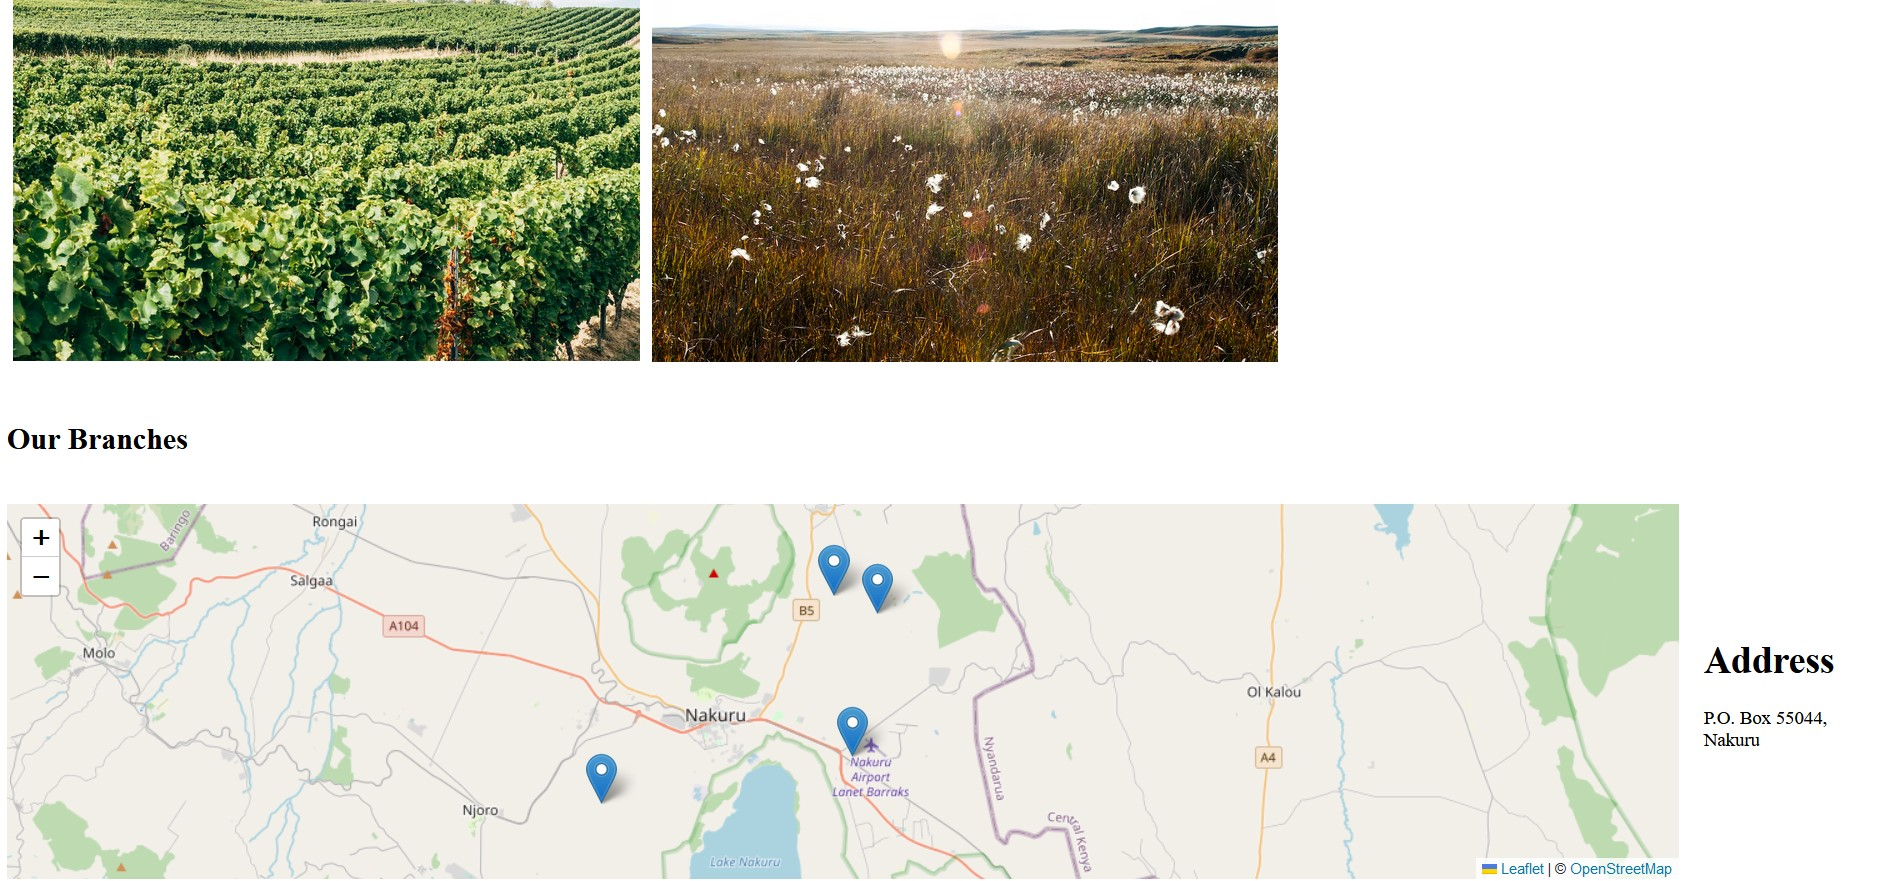
\includegraphics[width=26.21in]{../embedded}

Part of the success of making the webmap aligned to the left of our address text is the CSS property \texttt{display:\ flex}. This property aligns the element to fill or shrink according to the space available. The padding CSS property just creates space all around the element, thus creating a neat space between the leaflet map and the address text. Removing this will just make the address text and the leaflet map touch each other edge to edge.

The inspiration to place the map and text side by side was from this \href{https://www.w3docs.com/snippets/css/how-to-vertically-align-text-next-to-an-image.html?utm_source=pocket_saves}{site}.

Having done the above, you can consider you are as good a Leaflet mapper to undertake any task!

\begin{Shaded}
\begin{Highlighting}[]
\NormalTok{knitr}\SpecialCharTok{::}\FunctionTok{include\_graphics}\NormalTok{(}\FunctionTok{rep}\NormalTok{(}\StringTok{"https://images.unsplash.com/photo{-}1616588181775{-}138dc8ba4197?ixlib=rb{-}4.0.3\&ixid=MnwxMjA3fDB8MHxwaG90by1wYWdlfHx8fGVufDB8fHx8\&auto=format\&fit=crop\&w=1170\&q=80"}\NormalTok{))}
\end{Highlighting}
\end{Shaded}

\includegraphics{https://images.unsplash.com/photo-1616588181775-138dc8ba4197?ixlib=rb-4.0.3\&ixid=MnwxMjA3fDB8MHxwaG90by1wYWdlfHx8fGVufDB8fHx8\&auto=format\&fit=crop\&w=1170\&q=80}

\hypertarget{blocks}{%
\chapter{Blocks}\label{blocks}}

\hypertarget{equations}{%
\section{Equations}\label{equations}}

Here is an equation.

\begin{equation} 
  f\left(k\right) = \binom{n}{k} p^k\left(1-p\right)^{n-k}
  \label{eq:binom}
\end{equation}

You may refer to using \texttt{\textbackslash{}@ref(eq:binom)}, like see Equation \eqref{eq:binom}.

\hypertarget{theorems-and-proofs}{%
\section{Theorems and proofs}\label{theorems-and-proofs}}

Labeled theorems can be referenced in text using \texttt{\textbackslash{}@ref(thm:tri)}, for example, check out this smart theorem \ref{thm:tri}.

\begin{theorem}
\protect\hypertarget{thm:tri}{}\label{thm:tri}For a right triangle, if \(c\) denotes the \emph{length} of the hypotenuse
and \(a\) and \(b\) denote the lengths of the \textbf{other} two sides, we have
\[a^2 + b^2 = c^2\]
\end{theorem}

Read more here \url{https://bookdown.org/yihui/bookdown/markdown-extensions-by-bookdown.html}.

\hypertarget{callout-blocks}{%
\section{Callout blocks}\label{callout-blocks}}

The R Markdown Cookbook provides more help on how to use custom blocks to design your own callouts: \url{https://bookdown.org/yihui/rmarkdown-cookbook/custom-blocks.html}

\hypertarget{sharing-your-book}{%
\chapter{Sharing your book}\label{sharing-your-book}}

\hypertarget{publishing}{%
\section{Publishing}\label{publishing}}

HTML books can be published online, see: \url{https://bookdown.org/yihui/bookdown/publishing.html}

\hypertarget{pages}{%
\section{404 pages}\label{pages}}

By default, users will be directed to a 404 page if they try to access a webpage that cannot be found. If you'd like to customize your 404 page instead of using the default, you may add either a \texttt{\_404.Rmd} or \texttt{\_404.md} file to your project root and use code and/or Markdown syntax.

\hypertarget{metadata-for-sharing}{%
\section{Metadata for sharing}\label{metadata-for-sharing}}

Bookdown HTML books will provide HTML metadata for social sharing on platforms like Twitter, Facebook, and LinkedIn, using information you provide in the \texttt{index.Rmd} YAML. To setup, set the \texttt{url} for your book and the path to your \texttt{cover-image} file. Your book's \texttt{title} and \texttt{description} are also used.

This \texttt{gitbook} uses the same social sharing data across all chapters in your book- all links shared will look the same.

Specify your book's source repository on GitHub using the \texttt{edit} key under the configuration options in the \texttt{\_output.yml} file, which allows users to suggest an edit by linking to a chapter's source file.

Read more about the features of this output format here:

\url{https://pkgs.rstudio.com/bookdown/reference/gitbook.html}

Or use:

\begin{Shaded}
\begin{Highlighting}[]
\NormalTok{?bookdown}\SpecialCharTok{::}\NormalTok{gitbook}
\end{Highlighting}
\end{Shaded}


  \bibliography{book.bib,packages.bib}

\end{document}
